\documentclass{article}
\usepackage[UTF8]{ctex}
\usepackage{CJKutf8}
\usepackage{color}
\usepackage{natbib}
\usepackage{graphicx}
\usepackage{subfigure}
\usepackage{geometry}
\usepackage{amsmath}
\usepackage{mathrsfs}
% java code settings
\usepackage{listings}
\usepackage{xcolor}
\definecolor{dkgreen}{rgb}{0,0.6,0}
\definecolor{gray}{rgb}{0.5,0.5,0.5}
\definecolor{mauve}{rgb}{0.58,0,0.82}
\lstset{frame=tb,
     language=Java,
     aboveskip=3mm,
     belowskip=3mm,
     showstringspaces=false,
     columns=flexible,
     basicstyle = \ttfamily\small,
     numbers=none,
     numberstyle=\tiny\color{gray},
     keywordstyle=\color{blue},
     commentstyle=\color{dkgreen},
     stringstyle=\color{mauve},
     breaklines=true,
     breakatwhitespace=true,
     tabsize=3
}
\geometry{a4paper, scale=0.8}

\title{\textbf{EE447 Lab2 \\ Mesurement of WiFi Signal Strength\\ Report}}
\author{付昊源 517021910753}
\date{April 24, 2020}

\begin{document}

\maketitle

%%%%%%%%%%%%%%%%%%%%%%%%%%%%%%
\section{Lab Overview}
This lab aims to let us get used to the WiFi system and accomplish the sampling and measuring of WiFi signal strength through programming in Android on smartphone. We will design a Wifi scanning android app based on the given codes, as well as designing an indoor positioning system based on the detected signal strength.
\section{Lab Procedure}
This lab has already provided us with some basic codes with basic functions, so I will introduce my thoughts about the work flow first. Besides, since this lab needs us to design an algorithm for indoor positioning, I will also introduce my positioning strategy here and implementing details. Finally, I test my algorithm in my home and also design a GUI to visualize the positioning results for debug and test.

Note that my test environment is set at the living room of my home, and I used three wifis to scan and use for positioning, which include the router of my home, as well as my parents' mobilephone WiFi hotsopts.

\subsection{Understanding Initial Codes}
From the initial given codes, this app has already implemented the functions of scanning fixed SSID of WiFis' signal strength, show it at the GUI, write the scanning information into disk, and clean current data on the screen. In this subsection, I will analyze the work flow of the initial codes in brief.

The initial layout sets two buttons for 'SCAN' and 'CLEAN'. The first button is for detecting Wifi signal and the second button is to clear the current information. There is also an edit text for scanning results to show. Here I mainly introduce the work of 'SCAN' button. After clicking it, the app starts detecting the signal strength of some pre-defined SSIDs in SuperWiFi.java file. We can modify names in array \textit{FileNameGroup}. We also define some parameters such as test times, scanning time, as the private member variables here.

While the thread of scanning wifi is working, the work of MainActivity is blocked so that there is no data conflict and the return values are valid and meaningful. In scan thread, we first define the name of file to record each scan result, and write some basic information such as test ID and test date. All these info is for debug. Next, we continuously scan for \textit{scanningTime} times and record each result into the files above. Wifi signal is unstable, so we must scan for multiple times and treat the average value as its signal strength. After scanning, all information is stored and we can get it from some interfaces and show it in the edit view.

\subsection{Indoor Positioning Algorithm}
A natural idea is that the signal strength of a router is related to the distance from it. Actually, from the matrials I searched, the distance $d$ and the signal strength of a router, which is termed as $RSSI$, follow the equation below
\begin{equation} \label{rssi}
     d = 10 ^\wedge ((|RSSI|-A)/(10\times n))
\end{equation}
where $A$ is the absolute value of power at one meter distance to the router, and $n$ is path loss coefficient. These two parameters are related to environment and router type, and can be settled in this lab. Note that $RSSI$ is usually negative and Wifi signal strength is more powerful if $RSSI$ is bigger. However, $RSSI=0$ means there's no signal detected for the SSID.

There will be at least three routers for positioning, because one or two routers cannot ensure the actual position coordinates. The information we can pre-define includes the 2-d coordinates of three routers, $(x_1, y_1),(x_2,y_2),(x_3,y_3)$. After calculating three distances $d_1, d_2,d_3$ using equation \ref{rssi}, we can construct the following equations
\begin{equation} \label{distance}
\begin{aligned}
     (X-x_1)^2+(Y-y_1)^2&=d_1^2 \\
     (X-x_2)^2+(Y-y_2)^2&=d_2^2 \\
     (X-x_3)^2+(Y-y_3)^2&=d_3^2
\end{aligned}
\end{equation}
where $(X,Y)$ is the observer's or tester's coordinate. Of course it cannot always have valid solution, but we only consider valid scenario here.

\subsection{Algorithm Implement Details}
My test environment is set at the living room of my home, which is rather open and signal will seldom be weaken, so $n$ is set to 3.25, which is the lower bound of a meaningful $n$. For different WiFi, $A$ may be different, especially for routers and mobilephone hotsopt. From test I find $A=45$ for router and $A=55$ for mobilephone hotspot is the most accurate.

Besides, it is obvious that, in real condition, equation \ref{distance} may not have solution, which means three circles cannot always overlap at a single point. So in real experiment, I use some tricks to relax it. First, I use the upper two equations in \ref{distance} to calculate $(X,Y)$. In most cases, this will produce two results $(X_1,Y_1)$ and $(X_2,Y_2)$. Next, decide final coordinate by
\begin{equation}
\begin{aligned}
     i&=\arg\min_i|(X_i-x_3)^2+(Y_i-y_3)^2-d_3^2|, \quad i=1,2 \\
     (X,Y)&=(X_i,Y_i)
\end{aligned}
\end{equation}
Thus, we can get a sub-optimal coordinate $(X,Y)$.

\subsection{Visualization}
First of all, I add a 'VISUALIZE' button on the initial GUI, which can link to another page including canvas and some basic curves representing signal. The design is shown at Figure 1. I abstract the living room of my home as a $5m\times 3m$ rectangular, and place Wifi1 at position $(1,1)$, Wifi2 at $(1,4)$ and Wifi3 at $(2, 2.5)$. The data here is in meter.

\begin{figure}[htbp]
     \centering
     \subfigure[Initial GUI and  WiFi signal information after adding Visualization button.] {
         \begin{minipage}[t]{0.4\linewidth}
             \centering
             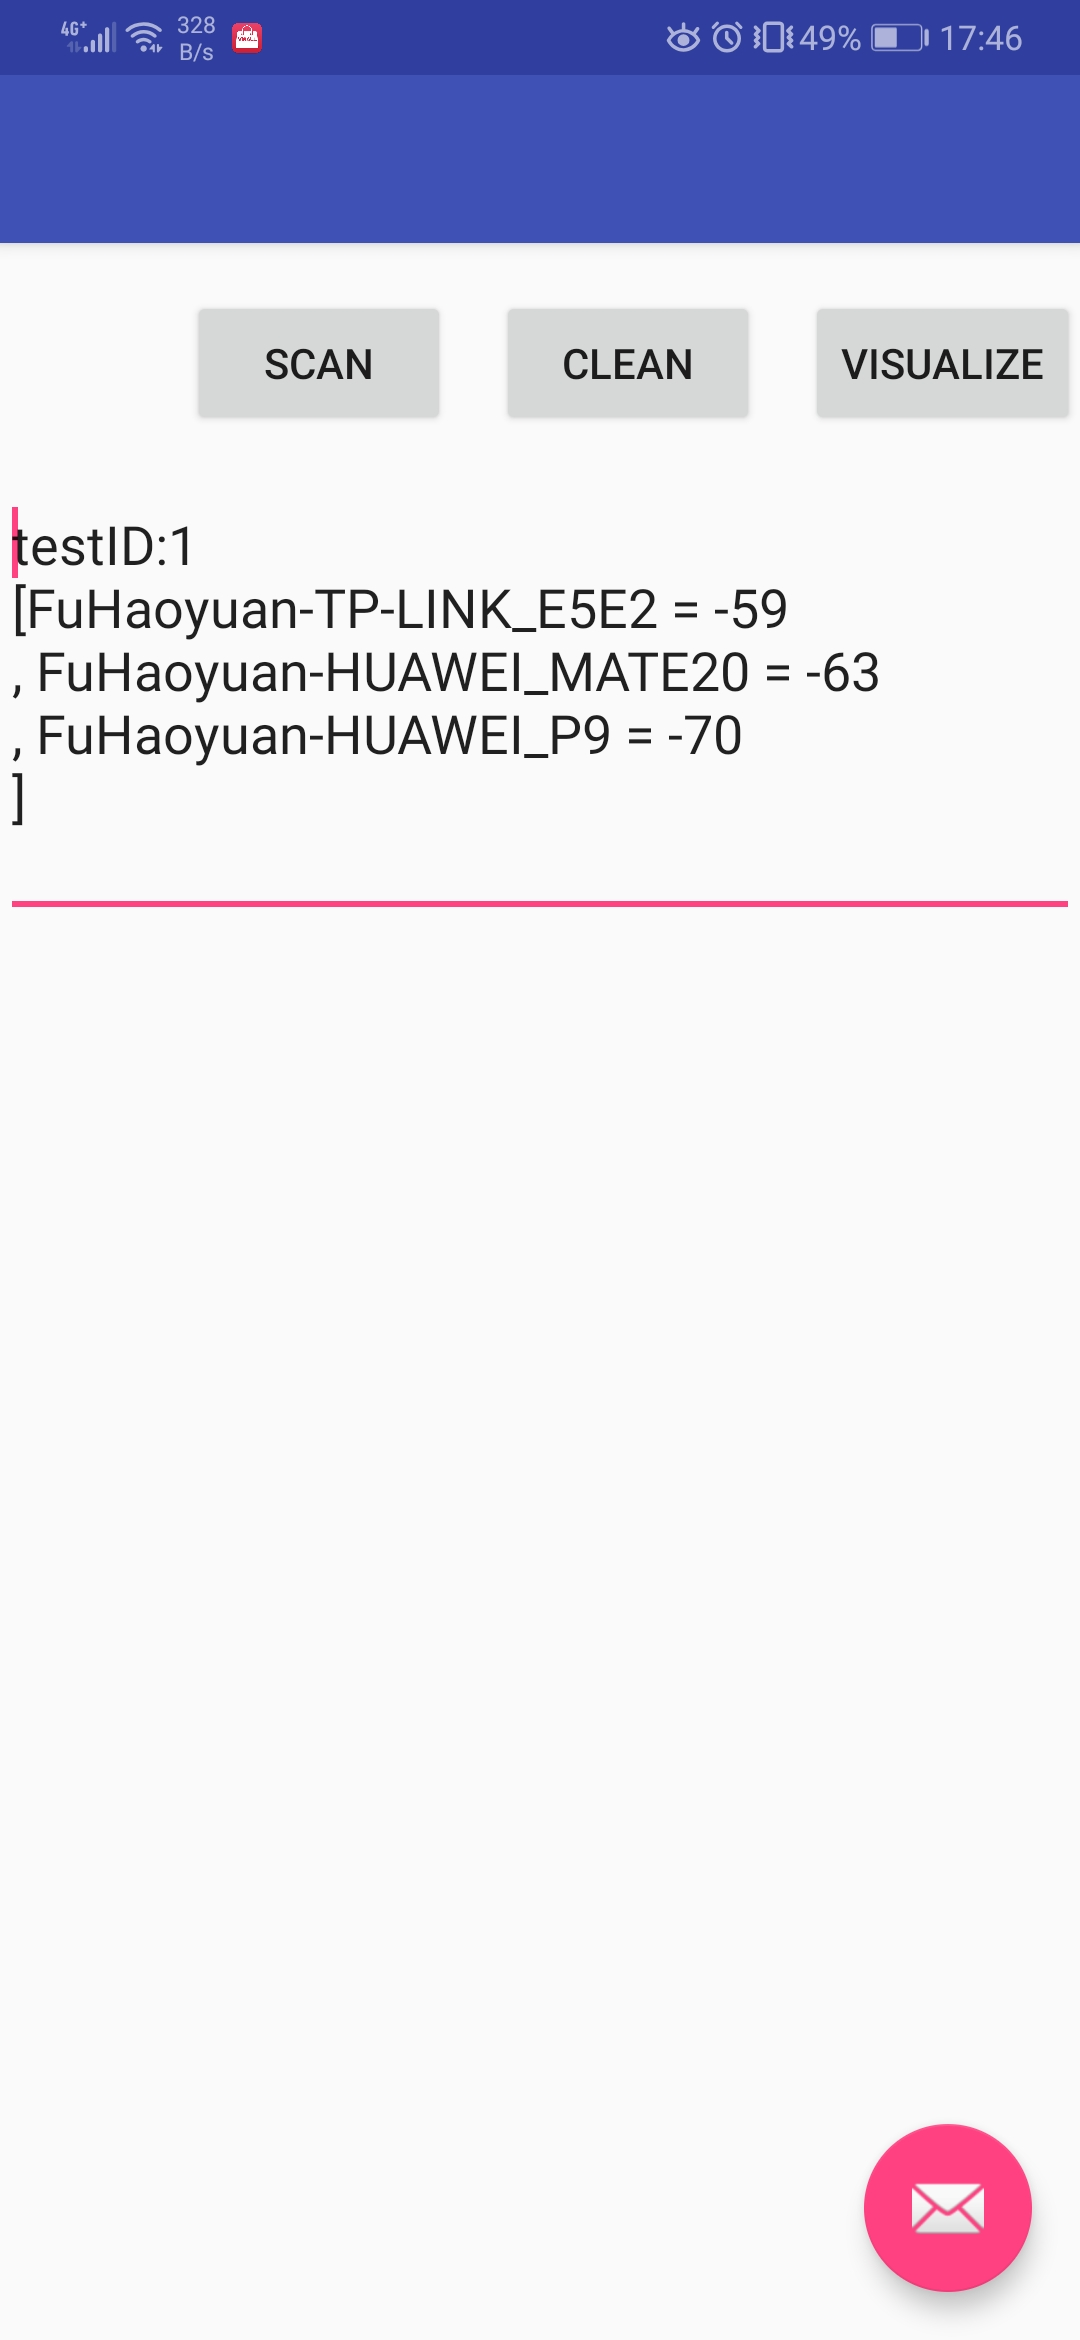
\includegraphics[width=\linewidth]{screen2.jpg}
         \end{minipage}
     }
     \subfigure[Visualization of three Wifis and positioning coordinate. Yello curve is for {\color{yellow}Wifi1}, green curve for {\color{green}Wifi2} and blue curve for {\color{blue}Wifi3}.]{
         \begin{minipage}[t]{0.4\linewidth}
             \centering
             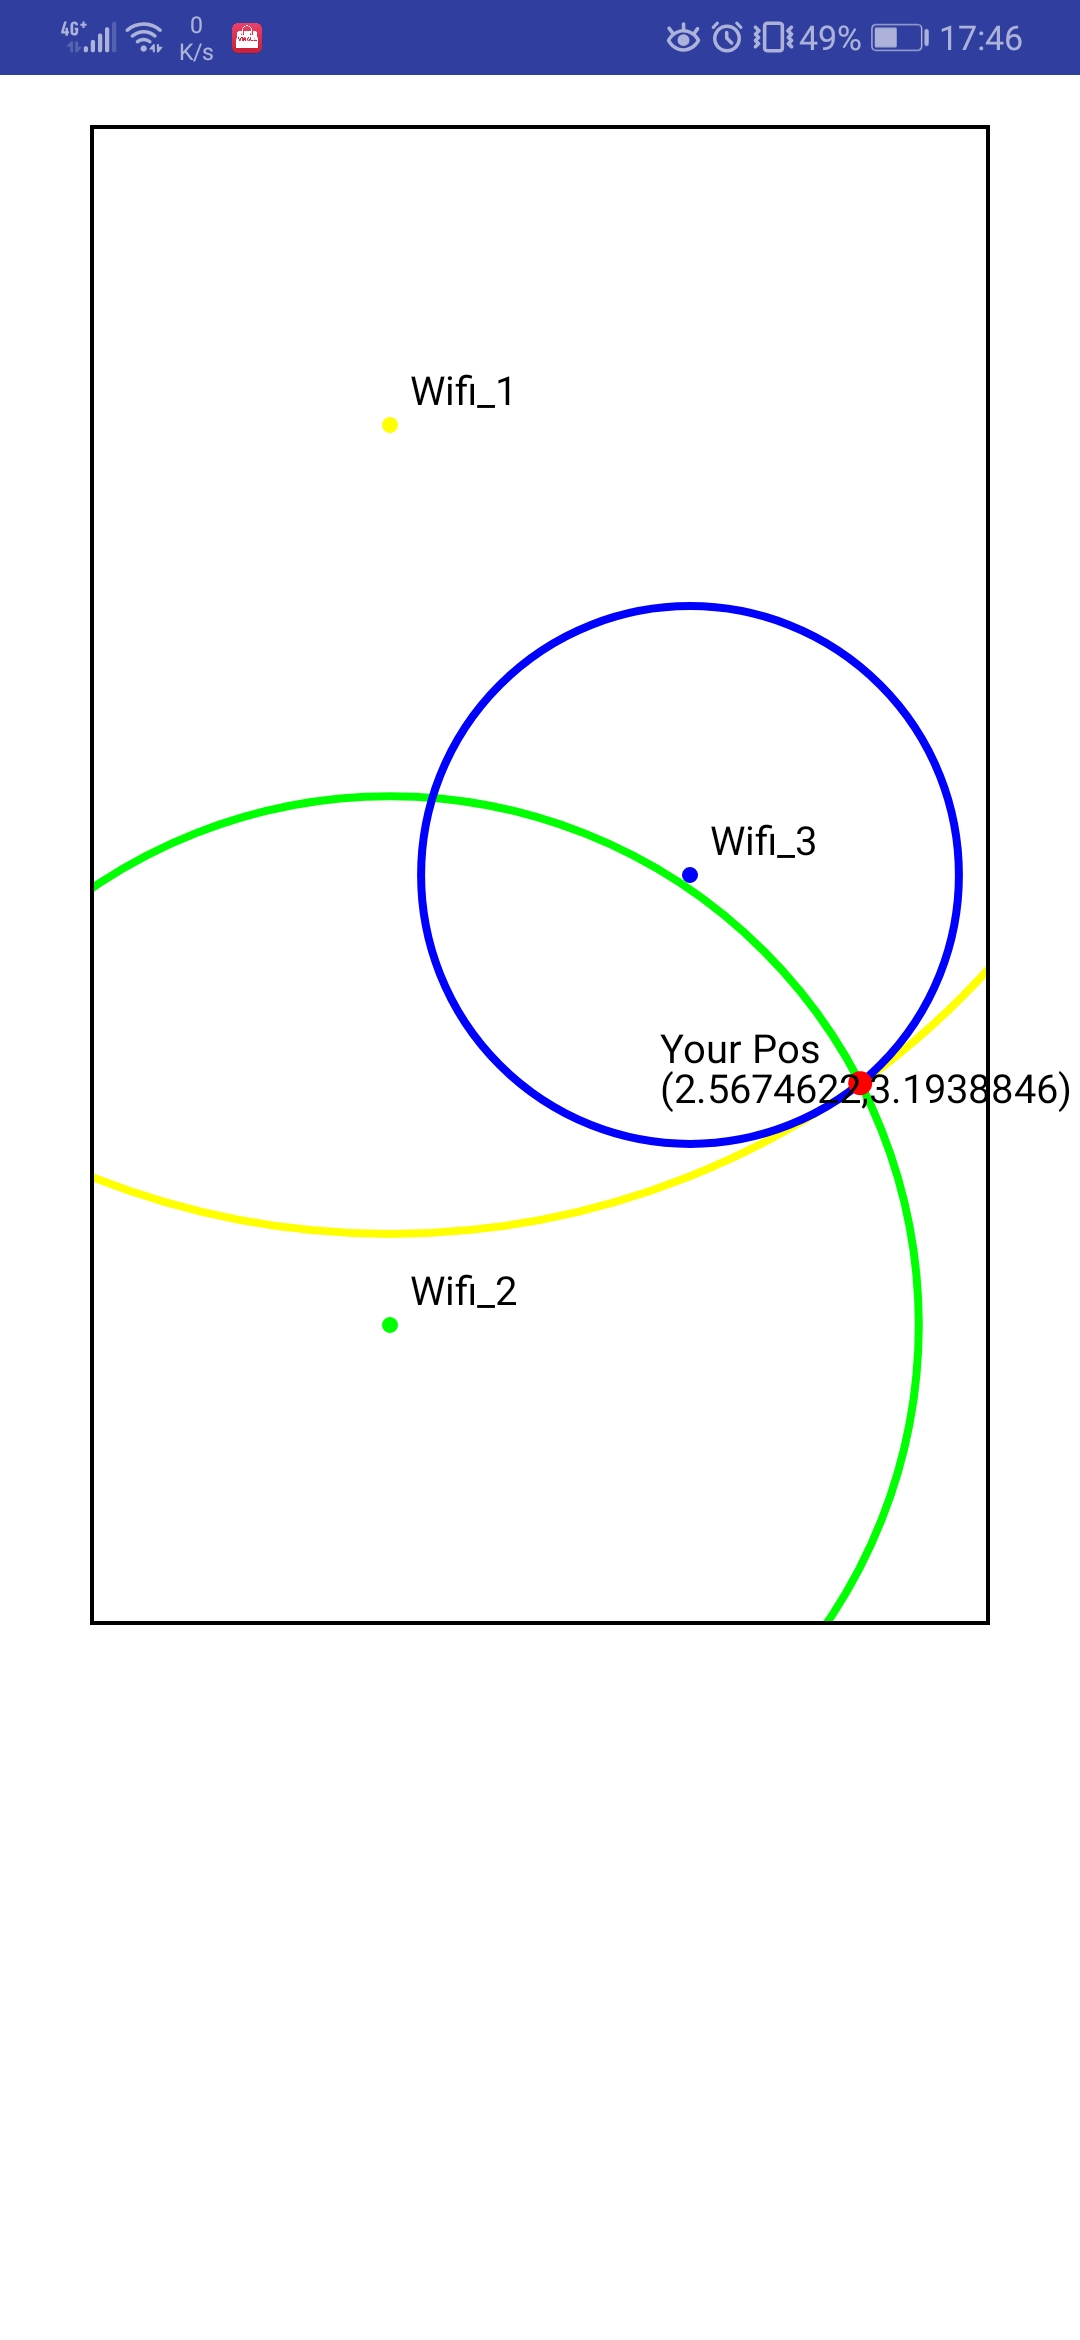
\includegraphics[width=\linewidth]{screen1.jpg}
         \end{minipage}
     }
     \caption{Screen shots of Measurement of WiFi Signal Strength on real mobilephone}
\end{figure}

In code implement, I use the \textit{android.content.Intent} as a sender and receiver between MainActivity and Visualization class. MainActivity adds data including positioning coordinate and three distances into the \textit{intent} and send it to Visualization class. Visualization class get data from \textit{intent} and draw curves as well as labeling keywords. The drawing procedure is similar to lab1, so I omit it here.

\section{Questions}

\subsection{Why is necessary to record all the measured value rather than only the average value?}
Only recording the average value will lose much information for debug. If the router signal is rather unstable, each value changes a lot, then this scan is meaningless and will produce much error. But if we only get the average value, we will miss these unstable data, and use a risky data for further positioning.

Besides, I also want to share an observation here. From checking the record file, I find that for the router in my home, though the pre-defined testing times is 10, there will be 20 results written into the file. After searching, I find that the SSID is not unique in a ScanResult, but the BSSID is unique. The router in my home is double-frequency, so it will have two BSSID and thus I will get 2 results about it in one test. If not for the record, I won't know things about BSSID.

\subsection{Besides the WiFi signal strength, what other information of the Routers can be got in the test?}
From Figure 2 we can see, besides the WiFi signal strength, information including center frequency, channel width, frequency, timestamp, BSSID, capability, SSID, etc can also be got in the test.
\begin{figure}[htbp]
     \centering
     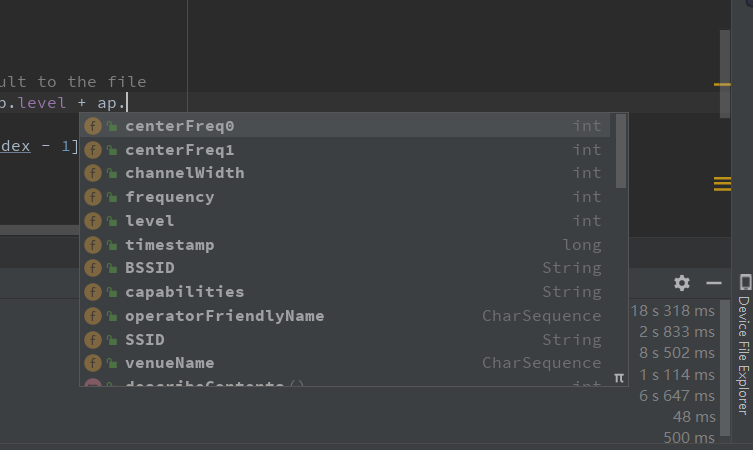
\includegraphics[width=0.7\linewidth]{extra_info.png}
     \caption{The options for scan results}
\end{figure}

\subsection{Why does scanning need to be operated in thread "scanThread"?}
I think there are two reasons for scanning to be operated in another thread. The first reason is that operating this procedure in a thread forces the CPU to operate this thread first instead of executing the codes in MainActivity. This is also friendly to synchronization. The second reason is that we can constrain the scanning time in a thread, so that the system won't busy wait, and this thread won't hold too much sources.

\section{Conlusion and Future Work}
In this lab, I mainly implement a positioning algorithm based on the distances calculated from scanning WiFi signal strength. I also visualize it on a canvas using some basic circles. From this lab I know the work flow of Wifi scanning procedure and relationship between RSSI and distance. I think the shortcoming of this algorithm is its inaccuracy, because Wifi signal strength is unstable itself. If we want to improve its accuracy, Wifi signal strength is the bottleneck.
%%%%%%%%%%%%%%%%%%%%%%%%%%%%%%

\end{document}
